\lhead{\begin{tikzpicture}[remember picture, overlay]
    \node [anchor=100,inner sep=0] (imagenIZQUIERDA) at (current page header area.north){
\includegraphics[width=18cm]{img/Encabezado.PNG}};
    \end{tikzpicture}}
    \rhead{Ángeles-Hurtado}
    \rfoot{\begin{tikzpicture}[remember picture, overlay]
    \node [anchor=140,inner sep=0] (imagenDERECHA) at (current page footer area.south){
\includegraphics[width=18cm]{img/Foot.PNG}};
    \end{tikzpicture}}
    %----------------------------------------------------------------------------------------
    \lfoot{ \thepage}
    % \renewcommand{\labelenumi}{\alph{enumi}.)} 
    %----------------------------------------------------------------------------------------
    %----------------------------------------------------------------------------------------
    %	TITLE SECTION
    %----------------------------------------------------------------------------------------
    
    \setlength{\droptitle}{-5\baselineskip} % Move the title up
    \title{\textbf{Estudio de tiempos y movimientos en el ensamble de un circuito electrónico utilizando diferentes métodos para su optimización }} % Article title
    
     \author{ 
     \textsc{Sáenz-Saavedra, Kenia Paola}\\ 
    %  Afiliación:
     \texttt{ Instituto Tecnológico de Querétaro } \\ 
     \texttt{Tecnológico Nacional de México} \\ 
     \texttt{Querétaro, México}\\ 
     \texttt{l22140911@queretaro.tecnm.mx} 
     \and 
     \textsc{Ángeles-Hurtado, Luis Alberto}\\ 
    %  Afiliación:
     \texttt{ Instituto Tecnológico de Querétaro } \\ 
     \texttt{ Tecnológico Nacional de México } \\ 
     \texttt{Querétaro, México}\\ 
     \texttt{alb3rt0.ah@gmail.com} 
    }
    
    
    %----------------------------------------------------------------------------------------
    
    % \begin{document}
    
    % Print the title
    \maketitle
    \thispagestyle{fancy}
    
    %----------------------------------------------------------------------------------------
    %	ARTICLE CONTENTS
    %----------------------------------------------------------------------------------------
    
    % \section*{Resumen}
    % \textit{Palabras clave:}
    % El resumen (ancho de página) deberá contener entre 100 y 200 palabras tipo Adobe Devangari 11 puntos.
    
    \begin{abstract}
    \noindent         
    \end{abstract}
    % 
    % 
    \textbf{\textit{Palabras clave}}: {Optimización, tiempo estándar.}
    % \keywords{First keyword should be the corresponding to the research area according with the authors guide. Maximum of 6 keywords.}
    \begin{itemize}
        \item Estándar, preciso, exacto, optimización, proceso.
    \end{itemize}
    
    \section{Introducción}
    
    %begin{itemize}
    
    El estudio de tiempos y movimientos es una herramienta la cual sirve para determinar los tiempos estándar de cada una de las operaciones que componen cualquier proceso, así como para analizar los movimientos que son realizados por parte de un operario para llevar a cabo dicha operación.
    
    A finales del siglo XIX, Frederick Taylor comenzó a estudiar los tiempos asociados con actividades laborales y desarrolló el concepto de tarea. Motivados por los estudios de tiempos de Taylor, alrededor del mismo periodo, la pareja de esposos Frank y Lillian Gilbreth condujeron estudios de movimientos (Krenn, 2011) que complementaron el trabajo de Taylor sobre estudios de tiempos.\cite{andrade2019estudio}
    
    El ensamble que se analizará en este estudio de tiempos es un circuito electrónico, este se puede definir como una colección de elementos eléctricos interconectados de alguna forma específica. Este circuito se estudiará a través de un Método de tiempos predeterminados por el grupo de 4to semestre de la carrera de ingeniería industrial. Consiste en una base de datos de tiempos de movimientos básicos.Se asignan tiempos estándar a los elementos básicos del trabajo. Se asignan a los movimientos fundamentales y a grupos de movimientos que no se pueden evaluar con precisión mediante los procedimientos ordinarios de estudio de tiempos con cronómetro. También son el resultado de estudiar una muestra grande de operaciones diversificadas con un dispositivo de ritmo como una cámara de filmación o vídeo-grabación, capaz de medir elementos muy cortos. \cite{parra2020analisis}
    
    El estudio que se realiza en este proyecto integrador tuvo cómo objetivo principal llevar a la práctica los conocimientos adquiridos a lo largo de estos 4 semestres, involucrando las materias y talleres ya cursados en la carrera. De igual manera a través de este ensamble desarrollar nuevas habilidades adquiridas en la materia de Estudió del Trabajo II. Aplicando lo anterior mencionado, obtener buenos resultados a través del estudio, buscando  una optimización en este proceso, que es buscar la mejor manera de realizar una actividad, lo más eficientemente posible, con la menor cantidad de recursos.
    
    El estudio de tiempos con cronómetro de forma tradicional, representa la técnica más utilizada como elemento de medición de las tareas, encontrándose más del 89\% de los trabajos desarrollados bajo ésta técnica.
    La aplicación del estudio de tiempos y movimientos sigue teniendo vigencia en la actualidad, como lo demuestran las 66 investigaciones realizadas entre los años 2010–2016, las cuales aplicaron las técnicas de medición del trabajo en sus formas tradicionales de muestreo del trabajo, estudio de tiempos con cronómetro y estándares de tiempo predeterminados.
    
    %endi{itemize}
     
    % Define estudio de tiempos y movimientos
    % define que es ensamble
    % define que es circuito electronico
    % define el metodo de tiempos predeterminados
    % define optimización
    % 
    % 
    \section{Justificación}
    
    %\begin{itemize}
    El entorno global ha llevado a las organizaciones a buscar la mejora de sus procesos por medio de la identificación y eliminación en forma gradual de las actividades que no generan valor a sus productos y procesos. Estas actividades representan costos operacionales que se traducen en despilfarros de tiempo, materiales, espacio y demás recursos organizacionales. Una de las técnicas más utilizadas para superar dichas deficiencias y elevar la productividad de los trabajadores es el estudio del trabajo. \cite{castiblanco2016que}
    Existen una diversidad de criterios para definir y de este modo clasificar a las empresas como micro, pequeñas, medianas y grandes, estos criterios son diferentes, dependiendo del país o entidad que las define y clasifica, aunque no se puede proporcionar un número exacto, se puede afirmar con seguridad que existen varios millones de empresas de manufactura a nivel global. La industria manufacturera es una parte crucial de la economía mundial, impulsando el crecimiento y el desarrollo económico en muchas regiones del mundo.\cite{saavedra2008caracterizacion}
    En diciembre de 2023, México contaba con 611.331 establecimientos relacionados con el sector manufacturero. El Estado de México era la entidad federativa con la mayor cantidad de locales de este tipo, albergando cerca del 11\% del total. El estado de Querétaro en México es un importante centro industrial y manufacturero, particularmente en sectores como la industria automotriz, aeroespacial, electrónica y de maquinaria. Aproximadamente, en Querétaro existen 7,0000 empresas de manufactura, considerando las unidades económicas registradas en censos y la información de diferentes organismos y clusters industriales. 
        
    
    %\end{itemize}
    % 
    % 
    \section{Descripción del problema}

   % \begin{itemize}
   %     \item Se debe describir la desviación o diferencia del %``es'' con respecto al ``debe ser''.
   %    \item Se debe hacer alusión a la incógnita científica*.
   %     \item Debe de tener Referencias científicas, URL, tesis, etc.
    %\end{itemize}
    
    %\textbf{*La incógnita científica es el elemento cuya solución incrementa el conocimiento científico.}
    Como ya se mencionó anteriormente, el objetivo principal del estudio de tiempos y movimientos es aumentar la eficiencia y reducir el desperdicio de tiempo y recursos en un proceso . Al analizar los procesos educativos, se pueden identificar las actividades que no agregan valor al aprendizaje y eliminarlas o simplificarlas.
    Los estudiantes, al tener la capacidad de realizar este proyecto desarrollaran capacidades y competencias que los posicionaran en un nivel como egresados.
    % 
    % 
    \section{Fundamentación teórica}
    
    %Es la parte medular y de mayor discusión, deberá ser la %fundamentación de la hipótesis, por tanto se deberá señalar %claramente la razón de la suposición y fundamentación de la %misma. Únicamente referencias científicas.
    %\begin{itemize}
     %   \item Se debe de retomar el tema que se planteo en la introducción, pero ahora profundizando para clarificar la incógnita científica y se pueda plantear la hipótesis.
      %  \item Se debe de retomar la descripción del problema, pero ahora a profundidad del (los) objeto(s) de estudio. 
       % \item Se debe de profundizar en las metodologías que se ha usado para el estudio del tema.
       % \item Referencias solo de artículos y libros científicos.
    %\end{itemize}
    El estudio de tiempos y movimientos es una herramienta crucial en la ingeniería industrial, especialmente en el ámbito de la manufactura de productos electrónicos, como los circuitos electrónicos. Este método se utiliza para analizar y optimizar los procesos de producción, mejorando la eficiencia y reduciendo los costos operativos. Involucra la medición detallada del tiempo que toma completar cada tarea en el proceso de ensamble. Este análisis permite identificar y eliminar ineficiencias, estableciendo estándares de tiempo para cada operación. Se enfoca en la simplificación y optimización de los movimientos necesarios para realizar una tarea. Se busca minimizar el esfuerzo y el tiempo empleado en movimientos innecesarios, mejorando la ergonomía y la productividad del trabajador.
    
    Algunos métodos de optimización son el (MTM) Que es el método de medición del tiempo. El MTM es una técnica que descompone cada operación en movimientos básicos y asigna un tiempo estándar a cada uno. Este método es particularmente útil para el análisis de procesos complejos como el ensamble de circuitos electrónicos. 
    También nos podemos encontrar con otro método como es la  Simulación y Modelado: La simulación mediante software como Simio permite modelar diferentes escenarios de producción y evaluar sus impactos en la eficiencia. Al simular el proceso de ensamble, es posible identificar cuellos de botella y probar diversas configuraciones de línea antes de implementarlas físicamente. \cite{breznik2023assembly}.
    
    De igual manera tenemos los Algoritmos Genéticos y Just-in-Time (JIT): La combinación de algoritmos genéticos con estrategias JIT optimiza la programación de la línea de producción y la alimentación de partes. Esto reduce tiempos muertos y exceso de inventario, mejorando la eficiencia global del proceso de ensamble. \cite{zhang2021research}.
    
    En la industria de ensamblaje de circuitos electrónicos, los estudios de tiempos y movimientos se aplican para:
    
   \begin{itemize}
       \item Balance de Línea de Ensamble: Distribuir equitativamente las tareas entre las estaciones de trabajo para minimizar los tiempos de ciclo y los periodos de inactividad. Esto se logra mediante el uso de herramientas como MTM y simulación.
       \item Optimización de Movimientos: Análisis detallado de los movimientos realizados por los operarios para ensamblar componentes, eliminando movimientos innecesarios y mejorando la disposición de las estaciones de trabajo para facilitar el acceso a herramientas y materiales. 
       \item Implementación de Sistemas JIT: Asegurar que los componentes y materiales necesarios lleguen justo a tiempo para ser ensamblados, reduciendo la acumulación de inventarios y los tiempos de espera. Esto se puede optimizar mediante simulaciones y algoritmos genéticos que ajusten dinámicamente las programaciones de producción.
       
    La metodologia de las 5´S es un sistema d eegstión de calidad y productividad originado en Japón cuyo objetivo es mejorar el ambiente de trabajo y la eficiencia organizacional. Esta metodología sigue un proceso establecido en cinco pasos, cuyo desarrollo implica la asignación de recursos, la adaptación a la cultura de la empresa y la consideración de aspectos humanos:
    
    \begin{itemize}
        \item Seiri (Clasificación): Consiste en separar lo neceario de lo innecesario y eliminar lo que no se necesita en el lugar de trabajo.
        \item Seiton (Orden): Implica organizar los elementos esenciales de manera sistematica y eficiente para facilitar su acceso y su uso. cada cosa debe tener un lugar especifico, lo que aumenta la productividad al reducir los tiempos de busqueda y movimineto, y mejora la seguridad al minimizar los obstaculos.
        \item Seiso ( Limpieza): Mantener un ambiente de trabajo limpio y ordenado para prevenir accidentes y mejorar la eficiencia. La limpieza debe de ser una responsabilidad compartida entre todos los empleados para asegurar un entorno laborar seguro y eficiente.
        
   \end{itemize}




    % 
    % 
    \section{Hipótesis}
    
   % Es la suposición con fundamento científico relativa a la solución del problema, necesidad o de cómo se aprovecha la oportunidad con la incógnita científica y se fundamenta con: 1. Una suposición (en afirmativo o negativo) y ésta deberá vincularse con:
    %2. La fundamentación científica que deberá ser precisa 3. Una entidad de comparación para probar la suposición y
    %4. La variable con que se califica o cuantifica la comparación o se prueba la hipótesis.
    Los alumnos elaborarán un proyecto integrador en el cual demostrarán los resultados obtenidos después de haber realizado un  análisis sobre el estudio de tiempos y movimientos, obteniendo el tiempo estándar. A partir de este proyecto adquirirán nuevas habilidades y competencias, así como también pondrán en practica las ya adquiridas a lo largo de los 4 semestres de clases.
    %\begin{itemize}
     %   \item Se debe de identificar claramente la suposición científica
      %  \item Se debe de identificar claramente el fundamento científico
       % \item Se debe identificar claramente la variable de respuesta
        %\item Se debe identifican claramente las realidades o modelos contrastantes
        %\item Se debe de establecer las variables asociadas, explicativas o que tienen relación funcional con la variable de respuesta
    %\end{itemize}
    % 
    % 
    \section{Objetivo}
    
    Realizar un estudio de tiempos y movimientos de un ensamble eléctrico para a partir de este análisis eliminar los movimientos ineficientes, eliminar tiempos muertos y aumentar la productividad, de esta manera comprobando la hipótesis planteada.
    
    
    \subsection{Objetivos específicos }
    
    \begin{itemize}
        \item Diseñar, mejorar e integrar sistemas productivos de bienes y servicios aplicando tecnologías para su optimización
        \item Diseñar, implementar y mejora sistemas de trabajo para elevar la productividad.
        \item Calcular el tiempo estándar que requiere un operador capacitado para el ensamblaje de un circuito electrónico.
        \item Desarrollar una guía de emergencia en la cual se establezcan los posibles riesgos de la locación donde se desarrolló el ensamblaje.
        \item Buscar la manera más económica de realizar la tarea.
        \item Realizar un estudio de tiempos y movimientos analizando todos los factores posibles.
    \end{itemize}
    
    
    % 
    \section{Metodología}
    
    
    %\begin{itemize}
    
    En la elaboración de este proyecto, es necesario establecer que se cumplirán con los objetivos descritos anteriormente. Para el diseño y la mejora en sistemas productivos, de manera sistemática se analizarán los procesos existentes, así como las instalaciones, herramientas, métodos, equipo y todos los factores que intervengan en este proceso de ensamblaje. Se identificarán áreas de mejora utilizando herramientas de análisis, en este caso se realizará un estudio de tiempos y movimientos. La obtención de la información y datos necesarios ,se realizó en el Instituto Tecnológico Nacional de México Campus Querétaro específicamente en el semestre enero-junio.
    
   Para el diseño, implementación y mejora de los sistemas se realizarán análisis detallados de los flujos de trabajo actuales, identificando cuellos de botella y oportunidades de mejora.Se pondrán en práctica nuevas metodologías de trabajo, como el trabajo en equipo colaborativo y la gestión ágil de proyectos.
   
    Se realizó la obtención de dos muestras continuas a partir de una cámara de video.  Continuando con el desarrollo de este proyecto, se llevaron a cabo las mejoras de propuestas y métodos utilizando metodologías ágiles, para determinar la medición del tiempo en ciclos.
    
    
    Se establecerán sistemas de retroalimentación para recopilar comentarios de los operarios que realizarán el ensamble para conocer sus incomodidades y retrasos en el proceso, así realizar los ajustes necesarios.Se aplicará el método de estudio de tiempos y movimientos para optimizar la eficiencia de las operaciones.
    %
    %
    \begin{figure}[H]
        \centering
        \includegraphics[scale=0.4]{32/img/diagramaMetodología.png}
        \caption{Diagrama de la metodología para la sección del desarrollo del sistema de clasificación.}
        \label{fig:enter-label}
    \end{figure}
    %
    %
    \begin{figure}[H]
        \centering
        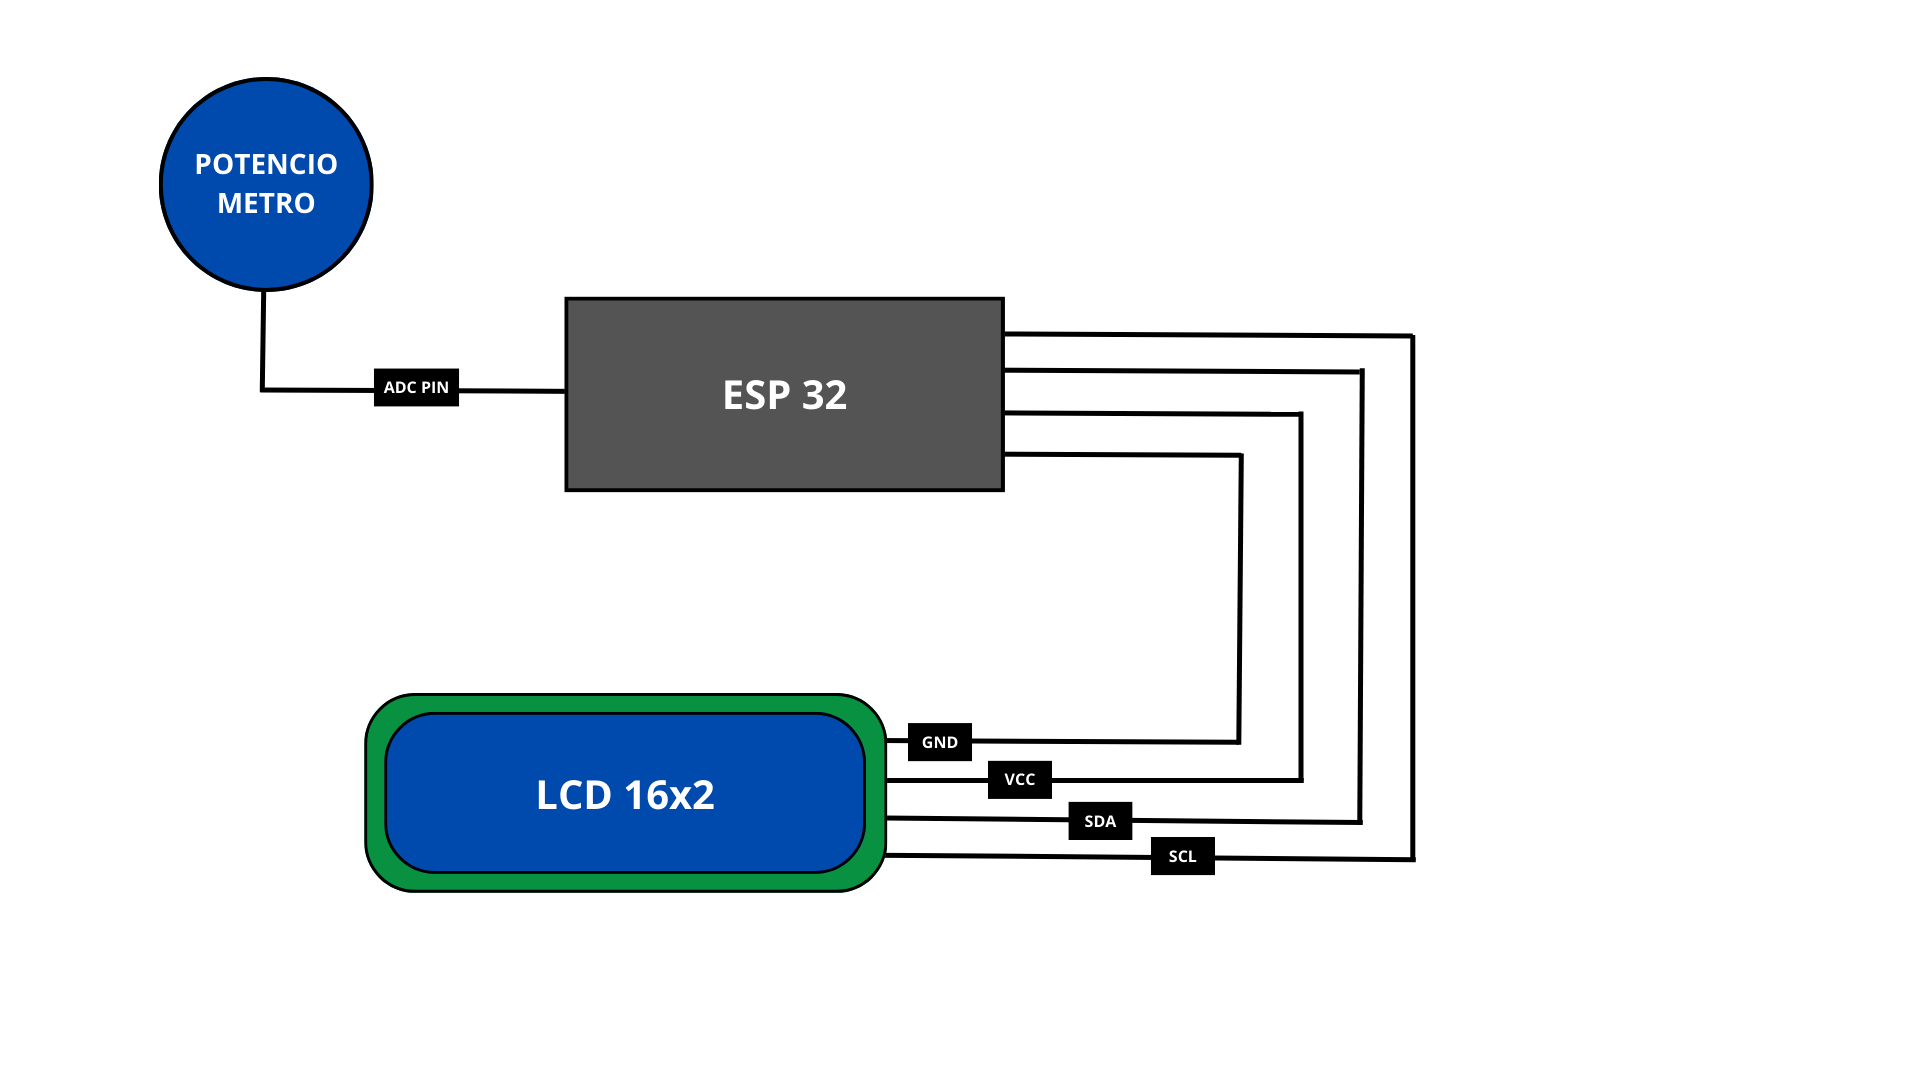
\includegraphics[scale=0.5]{32/img/cadenaDeMedida.png}
        \caption{Cadena De Medida}
        \label{fig:enter-label}
    \end{figure}
    %
    %
    \begin{figure}[H]
        \centering
        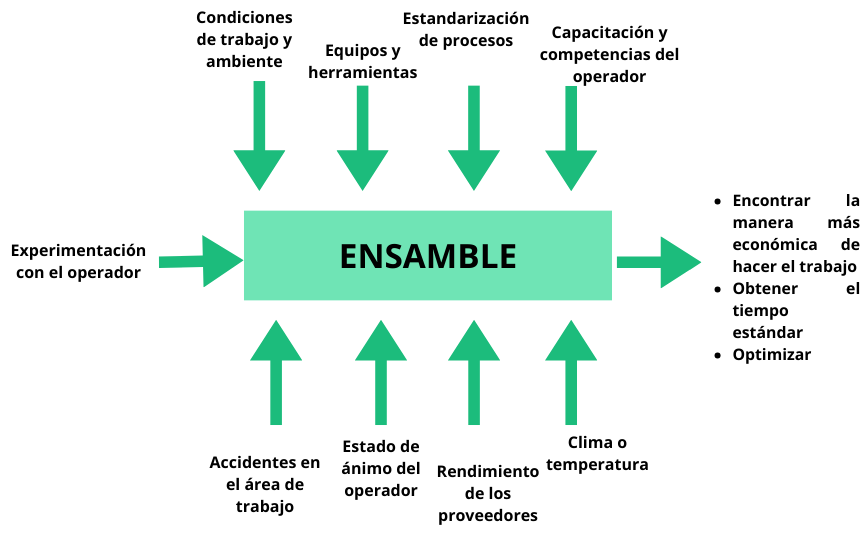
\includegraphics[scale=0.4]{32/img/diagramEntradasySalidas.png}
        \caption{Diagrama de entradas y salidas para ilustrar la relación entre los componentes des sistema y cómo interactúan entre sí.}
        \label{fig:enter-label}
    \end{figure}
    
    %
    %
    \subsection{Desarrollo de la guía de plan de emergencia} Un Plan de Acción de Emergencia en el contexto industrial es un documento integral que detalla los procedimientos y responsabilidades necesarios para garantizar la seguridad y el bienestar de los empleados y la protección de la propiedad durante una emergencia. Este plan generalmente incluye instrucciones detalladas para evacuaciones, refugio en el lugar, protocolos de comunicación y coordinación con los servicios de emergencia.
    En la elaboración de esta guía se hizo una recopilación de datos,
    se analizaron los procesos que se llevaban a cabo en la institución en caso de emergencia. A partir de esto se realizó una clasificación de riesgos internos y externos asignando una probabilidad de ocurrencia a cada uno de ellos . Posteriormente se realizó un programa de actividades de prevención de auxilio y se desarrolló un plan de acción, así como la identificación de capacidades. De igual manera se analizó el plano de localización de recursos, es decir, donde están localizada la señaletica o extintores de emergencia.
    Proseguimos con la identificación de riesgos externos y de puntos de reunión, tambien se desarrolló una brigada de evacuación y se estableció un directorio telefónico de emergencia.
    %
    \subsection{Análisis de los métodos, materiales, herramientas e instalación utilizada en la ejecución del ensamble de un circuito eléctrico.}

    Cómo mencionamos anteriormente, es necesario analizar cada uno de los factores que intervienen en nuestro proceso de ensamblaje 

    \subsubsection{Planeación}
    
    En el proceso de elaboración de este proyecto, primeramente se planteó el objeto de estudio que se utilizaría para realizar esta experimentación, que es un circuito eléctrico conformado por una tarjeta LCD y un ESP-32.Como primer paso, nos familiarizamos con los componentes de este ensamble. A continuación se muestran todos los componentes de nuestro ensamble, especificando modelo y costo por unidad. Vease la tabla \ref{fig:lista-materiales}
    \begin{figure}[H]
        \centering
        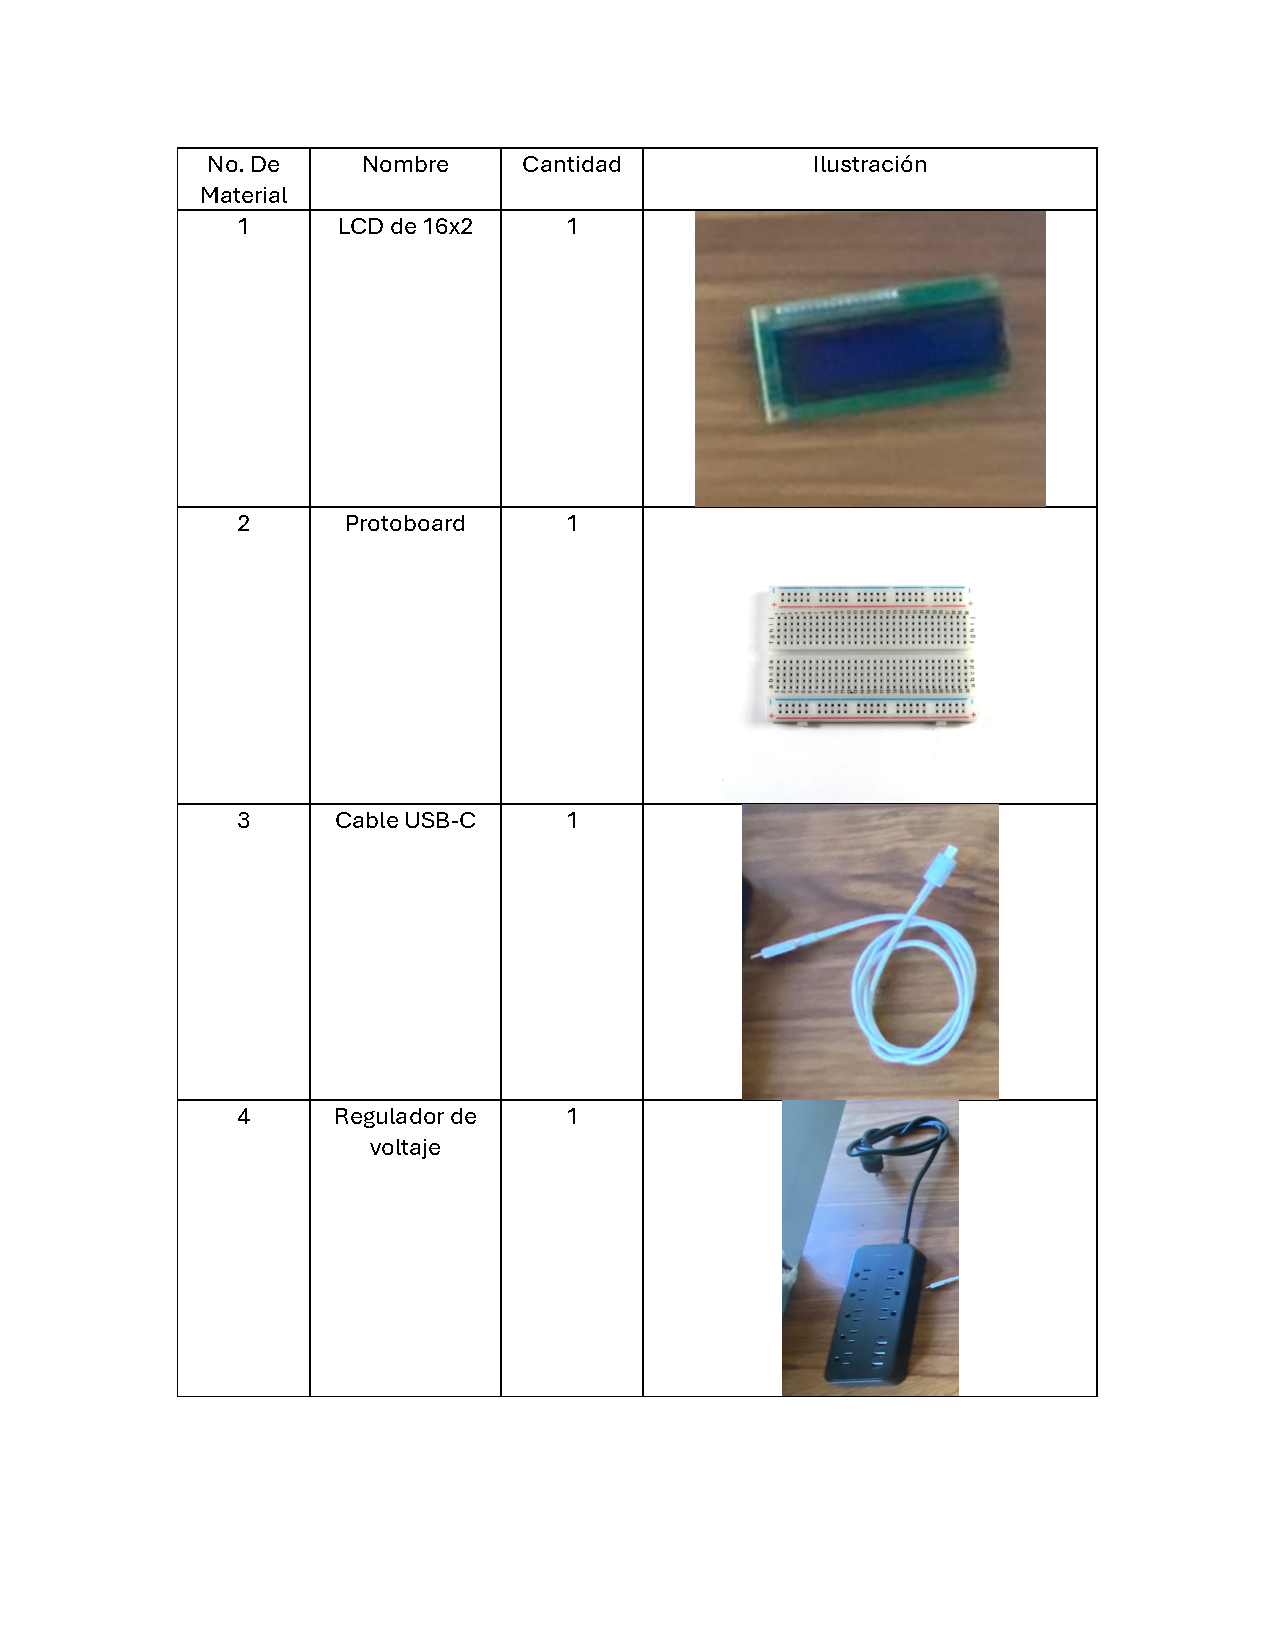
\includegraphics[scale=0.4]{32/img/listaDeMateriales.pdf}
        \caption{Lista de materiales empleados en el ensamble}
        \label{fig:lista-materiales}
    \end{figure}
%
%
Cada uno de los materiales se deben medir, tocar, oler y todo lo necesario para a partir de esto, plasmarlos en algún programa asistido por computadora especificando las medias de cada uno, en este caso se utilizó Solid Works en la versión 2019. Es necesario describirlos en sus totalidad.

\begin{itemize}
    \item Protoboard 300 p
    %
    \begin{figure}[H]
        \centering
        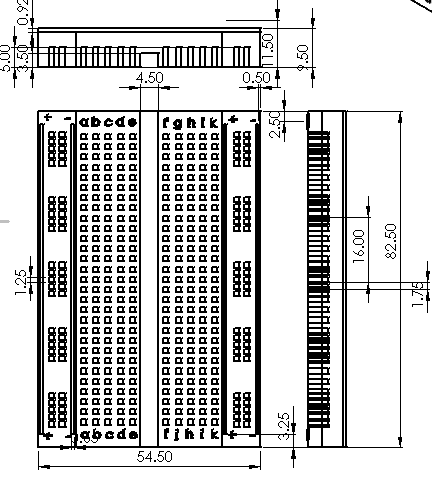
\includegraphics[scale=0.7]{32/img/protoboardCotas.PNG}
        \caption{Dibujo acotado de Protoboard}
        \label{fig:enter-label}
    \end{figure}
    %
    
     El protoboard utilizado en este ensamble es una placa que se utiliza para construir prototipos de circuitos electrónicos sin necesidad de soldar. La versión de 300 puntos es más pequeña, ideal para proyectos simples o para pruebas rápidas.Tiene 300 puntos de conexión, organizados en filas y columnas con carriles de alimentación en los bordes. Está  hecha de plástico ABS con tiras de contactos de cobre o latón recubiertas de níquel.
     %
     %
    \item ESP32-C6-WROOM-1
    Usado para desarrollar aplicaciones IoT, controladores embebidos, y proyectos que requieran conectividad inalámbrica.Está hecha de placa de circuito impreso (PCB) con componentes electrónicos como el microcontrolador, antena, y otros circuitos integrados.
    %
    \begin{figure}[H]
        \centering
        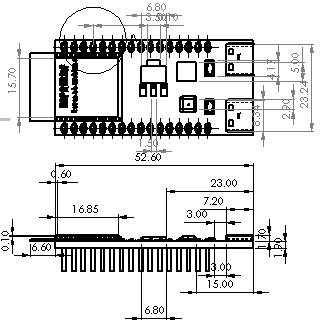
\includegraphics[scale=0.9]{32/img/esp32Cotas.PNG}
        \caption{Dibujo acotado de ESP 32}
        \label{fig:enter-label}
    \end{figure}
    %
    %
    \item LCD Display 16x2 
    Es una pantalla de cristal líquido con 16 columnas y 2 filas de caracteres. Generalmente con retroiluminación LED. Su propósito es mostrar información alfanumérica en proyectos electrónicos, como datos de sensores o mensajes del sistema. Los materiales de los que stá compuesto son vidrio LCD, electrodos de indio y estaño, retroiluminación LED, y carcasa de plástico.
    %
    \begin{figure}[H]
        \centering
        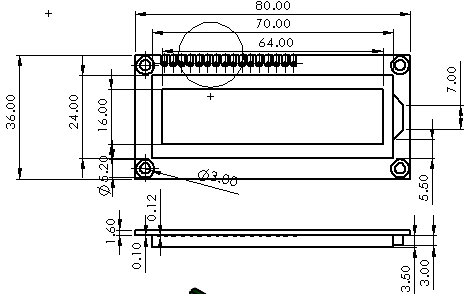
\includegraphics[scale=0.7]{32/img/lcdCotas.PNG}
        \caption{Caption}
        \label{fig:enter-label}
    \end{figure}
    
    \item Potenciómetro 3540S-1-501L
     Este es un potenciómetro de precisión con un valor de resistencia de 500 ohmios y un diseño robusto. Su propósito es ajustar la resistencia en un circuito, permitiendo el control de variables como el brillo de una pantalla o el volumen de un sonido. Está hecho a partir de carcasa de plástico o metal, elemento resistivo (generalmente de carbono o cermet), y contactos metálicos.
     %
     \begin{figure}[H]
         \centering
         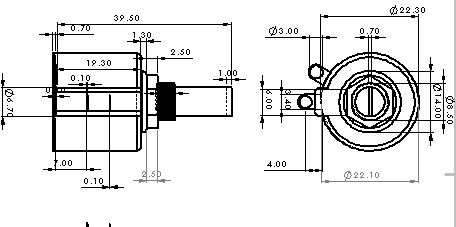
\includegraphics[scale=0.7]{32/img/potenciometroCotas.PNG}
         \caption{Caption}
         \label{fig:enter-label}
     \end{figure}
     %
     %
    \item Módulo SPI 12C
     Es un adaptador o convertidor que permite la comunicación entre dispositivos usando los protocolos SPI (Serial Peripheral Interface) e I2C (Inter-Integrated Circuit). Su objetivo es facilitar la conexión y comunicación entre microcontroladores y periféricos como sensores, memorias, y pantallas.Los materiales que lo componen son PCB con componentes electrónicos como convertidores de nivel lógico y conectores.
     %
    

    \item Regulador de voltaje
     Componente que mantiene una salida de voltaje constante independientemente de las variaciones en la entrada o en la carga.Su propósito es proveer una tensión estable a los circuitos electrónicos, protegiéndolos de sobrevoltajes y fluctuaciones.En este caso, el regulador que utilizamos cuenta con 8 salidas, 3 USB y una tipo C. Los materiales que lo componen son semiconductores (transistores, diodos), encapsulado de plástico o metal, y contactos metálicos.
     
    \item Cable USB-C
    Este es un cable de conexión con conector USB-C en un extremo, conocido por su reversibilidad y alta velocidad de transferencia de datos. Su propósito es transferir datos y energía entre dispositivos como teléfonos, computadoras, y periféricos. Está hecho a base de conductores de cobre, aislamiento de plástico, y conectores metálicos.
    
    \item Resistencias
    Estas son componentes electrónicos que limitan el flujo de corriente en un circuito. Las que utilizaremos en este ensamble son de 330 ohms. Su propósito es controlar la corriente y dividir voltajes en circuitos electrónicos. Están hechas a base de un cuerpo cerámico o de vidrio con una película de carbono o metal, y terminales de alambre de cobre.

    \item Cables Dupont-10 Macho-macho
    Conjunto de cables con conectores macho en ambos extremos, de 10 cm de longitud. Utilizado para conectar componentes en protoboards o entre módulo. Utilizaremos 4 de estos en distintos colores.Están compuestos por conductores de cobre, aislamiento de plástico, y conectores metálicos.
    %
    \begin{figure}[H]
        \centering
        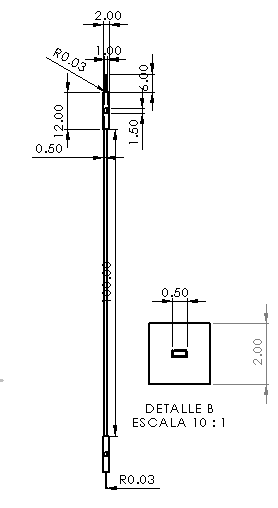
\includegraphics[scale=0.7]{32/img/dupontMMCotas.PNG}
        \caption{Dibujo acotado de cables dupont MM}
        \label{fig:enter-label}
    \end{figure}
    %
    %
    \item Cables Dupont-10 Hembra-Macho
    Conjunto de cables con un conector hembra en un extremo y un conector macho en el otro, de 10 cm de longitud.Sirevn para conectar componentes con pines hembra a otros con pines macho, facilitando la interconexión en protoboards y módulos.
    %
    \begin{figure}[H]
        \centering
        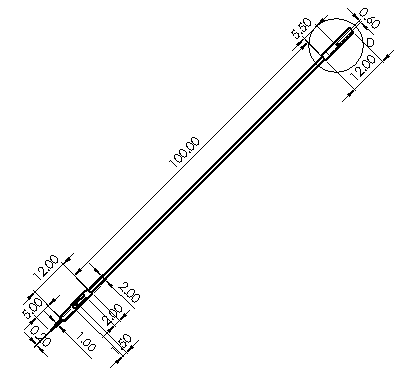
\includegraphics[scale=0.7]{32/img/dupontHembraMachoCotas.PNG}
        \caption{Dibujo acotado de Cables Dupont HM}
        \label{fig:enter-label}
    \end{figure}

    \item Almohadilla para soldar
    Superficie resistente al calor utilizada como base para soldar componentes electrónicos.Su función es proteger la mesa de trabajo del calor y proporcionar una superficie adecuada para el proceso de soldadura. De igual manera sirve para organizar los elementos del ensamble que se llevara a cabo, ya que está dividido en subsecciones de distintos tamaños.Está hecha a base de silicona o caucho resistente al calor.
\end{itemize}
    
    
     Posteriormente, se elaboró un manual en dónde se describe cada herramienta, equipo, maquina y todos los pasos detalladamente necesarios que el operador debe de seguir para llegar al ensamble final.
     Una vez realizado nuestro manual, se planeó realizar dos muestras con cámara de video en el cual el operador realice el ensamble. La toma de estas muestras deben llevarse a acabo en diferentes días y de preferencia en diferentes contextos, es decir, diferentes horas, con distintos climas etc. En este caso el analista debe de tener el menor contacto posible con el operador.
     Una vez obtenidas estas muestras se comienza con el desarrollo del proyecto, en el cual se planea que los analistas compartan los datos obtenidos y así determinar el tiempo estándar en el que un operador competente realice el trabajo a un ritmo normal.Para llegar a este resultado se  implementarán las mejoras y modificaciones pertinentes, como es la aplicacion de las 5 S. De igual manera se realizará un analísis de costos para determinar la manera más economica de realizar el trabajo
     %
     %
    \subsubsection{5´S}
    La aplicación de las 5´S en este proceso de ensamblaje es de suma importancia para mantener nuestro lugar de trabajo organizado, limpio y eficiente. Esto ayudará a mejorar la eficiencia, la seguridad y la calidad de nuestro ensamble final. A continuación se explica la manera en la que se sugiere aplicar esta metodologia en nuestro contexto:
    %
    %
    
    \begin{enumerate}
     \item Clasificación: 
        Se identificará y clasificarán todos los componentes y herramientas para el ensamble del circuito eléctrico. Se eliminará del área de trabajo cualquier cosa que no sea necesaria, así cómo componentes defectuosos y herramientas que no sean relevantes.
        \item Orden:Se colocarán los comoponentes, herramientas en lugares designados y etiquetados para que sean fáciles de encontrar y acceder ahorrando tiempo en la busqueda.
        \item Estandarización: Se desarrollaran procedimientos estandarizados para la clasificación, organización y limpieza. Se sugiere crear listas de verificación y hacer las correcciones pertinentes al manual de procedimientos.
        \item Disciplina: Se capacitará y motivará al operador para que siga los procedimientos establecidos, realizando supervisiones regulares para asegurar el cumplimiento de estas.
        
    \end{enumerate}
    
    \end{itemize}
    %
    %
    \subsubsection{Desarrollo de sistemas de tiempo predeterminado}
    %
    
    Para el desarrollo de los STP debemos de seguir una serie de pasos que están basados en los Therbligs. Deben ser aplicados por un analista capacitado para así predecir con precisión el tiempo necesario para hacer un trabajo. Esto se hace con la finalidad de realizar un análisis de métodos para determinar un  Estos se dividen en 3 pasos:
    %
    %
    \begin{itemize}
        \item Dividir el trabajo en elementos.
        %
        Todos los movimientos que realice el operario se dividen en 10 categorias que son las siguientes:Alcanzar, mover, girar, aplicar presión, asir, colocar,soltar,separar, movimientos de cuerpo y movimientos de ojos.
    
    \item Asignar valores de tiempo a cada elemento.
    %
    Para la asignación de valores utilizamos el TMU que son las Unidades de Medida de Tiempo. 
    \begin{figure}[H]
        \centering
        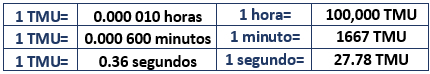
\includegraphics[scale=0.7]{32/img/tablasTMU.png}
        \caption{Unidades de Media de Tiempo}
        \label{fig:enter-label}
    \end{figure}
    %
    %
    Cómo sabemos la acción de "alcanzar" se subdivide en 5 casos. 
    \begin{figure}[H]
        \centering
        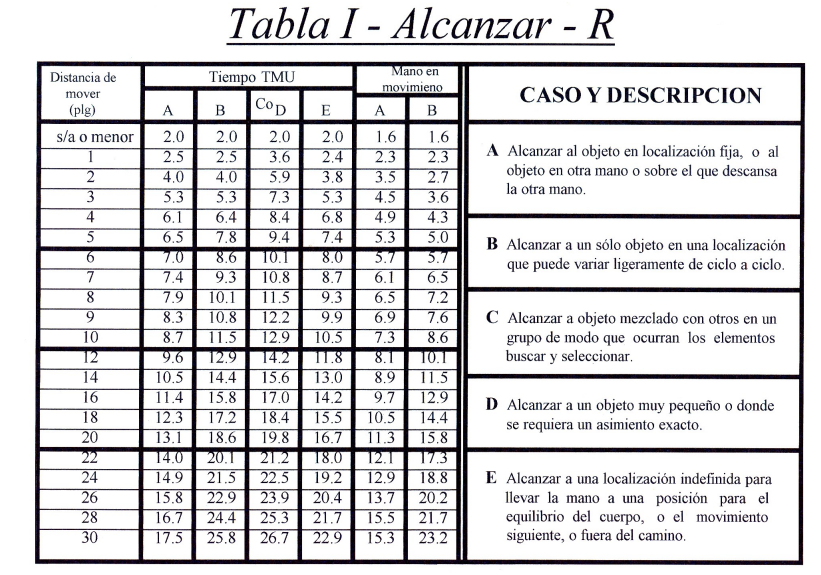
\includegraphics[scale=0.3]{32/img/tablaIAlcanzar.png}
        \caption{Tabla I Alcanzar R}
        \label{fig:enter-label}
    \end{figure}
    
    Aquí podemos observar la tabla\cite{bibiano2022automatizacion}

    Por otro lado, la acción de mover se subdivide en 3 casos, aquí se debe de considerar la relación con el peso del objeto o con su resistencia al movimiento.
    %
    \begin{figure}[H]
        \centering
        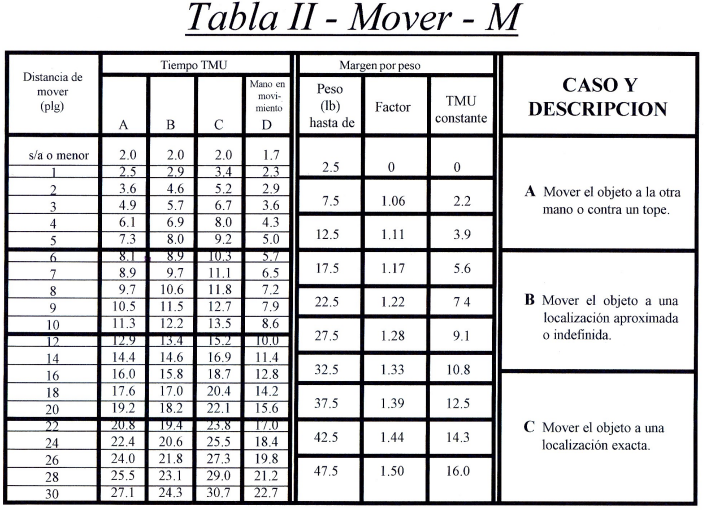
\includegraphics[scale=0.41]{32/img/tablaIIMover.png}
        \caption{Caption}
        \label{fig:enter-label}
    \end{figure}
    %
    \begin{figure}[H]
        \centering
        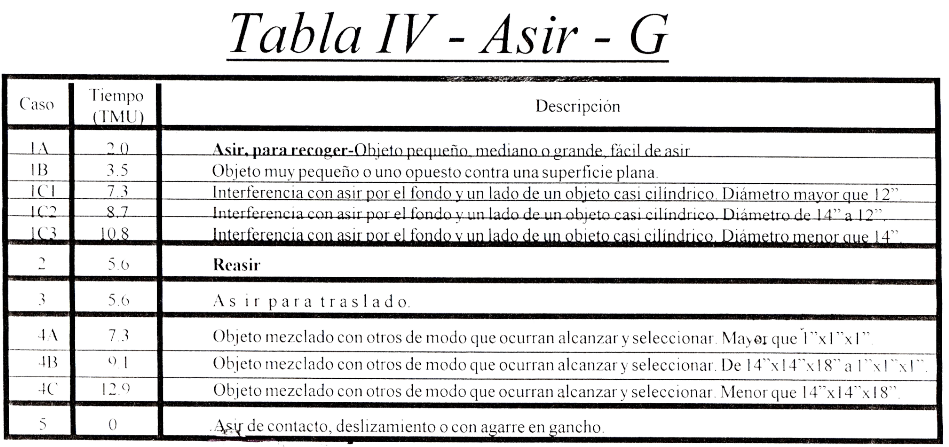
\includegraphics[scale=0.31]{img/tablaAsir.png}
        \caption{Tabla Asir}
        \label{fig:enter-label}
    \end{figure}
    %
    %
    \begin{figure}[H]
        \centering
        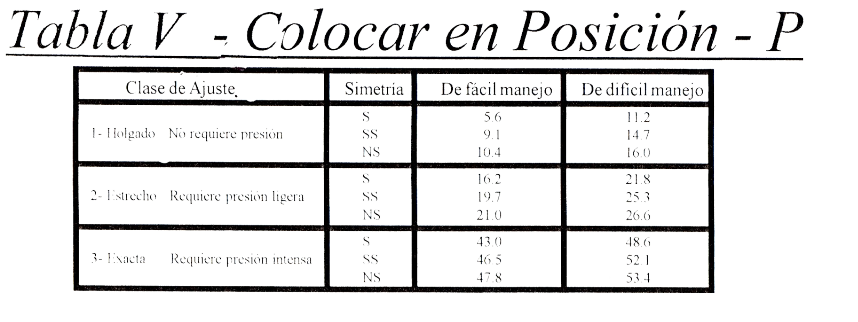
\includegraphics[scale=0.31]{img/tablaColocar.png}
        \caption{Tabla Colocar}
        \label{fig:enter-label}
    \end{figure}
    
    \item Sumar los tiempos de todos los elementos
    \end{itemize}
    Después de haber clasificado todos los movimientos y haberle asignado un valor a cada uno de ellos, se realiza la suma de todos estos movimientos
        
    \subsubsection{Desarrollo de muestreo de trabajo}
    %
    %
    En esta sección el meustreo de trabajo lo podemos considerar como una herramienta para disminuir el costo que se presenta en el estudio del tiempo. 
    
    \subsubsection{Datos estándar continuos y discretos}
    %
    %
    \subsection{Diseño de la forma más económica de realizar el trabajo}
    %
    %
    \subsection{Normalización de métodos, materiales, herramientas e instalaciones}
    %
    %
    \subsection{Determinación del tiempo estándar para que un operador competente realice el trabajo con marcha normal}
    
    
    
    %\end{itemize}
    
    

    


    
    \section{Resultados y discusión}
    \subsection{Desarrollo de la guía de emergencia}
    
    Con la finalidad de eliminar todos los posibles riesgos de emergencia e incendio, se realizó esta guía de plan de emergencia. De igual manera se implementaron nuevas estrategias como es la capacitación constante del personal de como actuar en caso de una emergencia, esto con la finalidad de que en caso de ocurrencia sepan como actuar, tomen las mejores decisiones y salvaguarden la integridad fisica de todas las personas en riesgo. 
    A continuación se describe la ubicación y datos generales donde se llevó a cabo el ensamble para posteriormente analizar lo antes planteado.
    \begin{figure}[H]
        \centering
        \includegraphics[scale=0.4]{32/img/ubicaciónDelInstituto.png}
        \caption{Av Tecnológico S/N, Centro Histórico, Centro, 76000 Santiago de Querétaro, Qro.}
        \label{fig:enter-label}
    \end{figure}
    %
    %
    \begin{figure}[H]
        \centering
        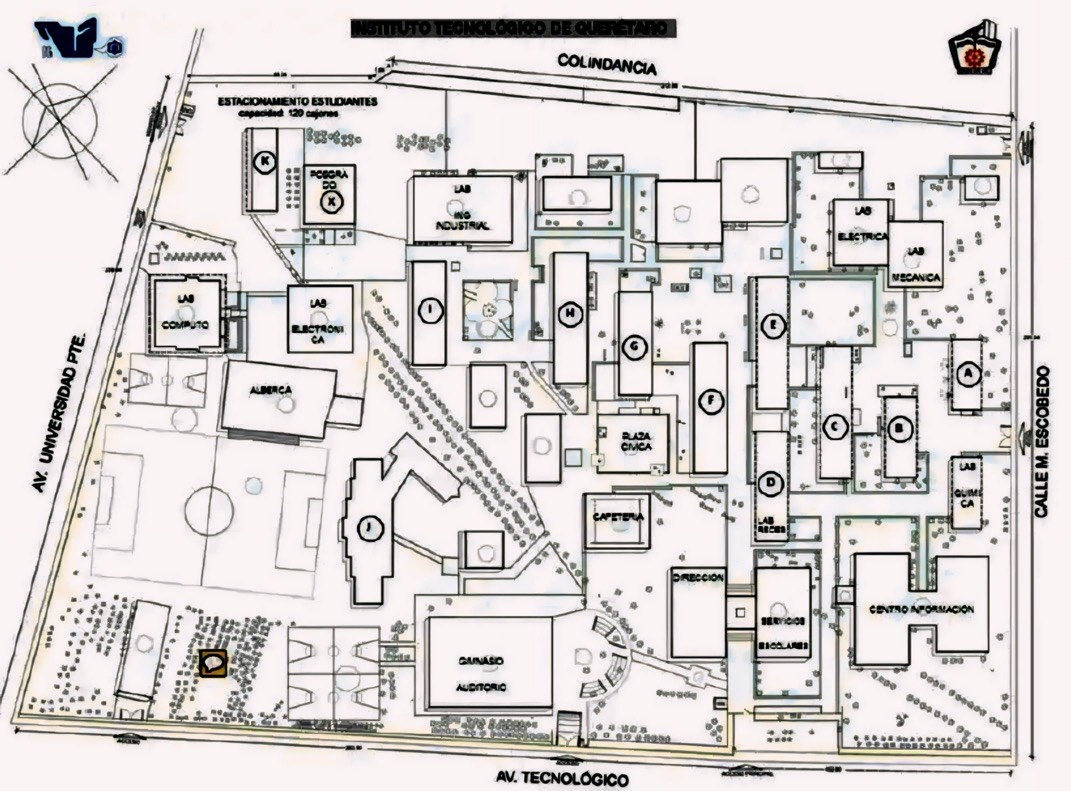
\includegraphics[scale=0.2]{32/img/croquisITQ.jpg}
        \caption{Croquis Instituto Tecnológico de Querétaro}
        \label{fig:enter-label}
    \end{figure}
    \subsubsection{Identificación del Riesgo}
    Se presenta un análisis detallado de la identificación de riesgos realizada durante el desarrollo del plan de emergencia. Este análisis incluye una evaluación sistemática de los riesgos internos y externos que pueden afectar la operatividad y seguridad de la industria. Véase el diagrama  \ref{fig:identificacion-riesgos}

    %
    %
    \begin{figure}[H]
        \centering
        \includegraphics[scale=0.25]{32/img/diagramaIdentificaciónDeRiesgos.png}
        \caption{Diagrama para la identificación de riesgos}
        \label{fig:identificacion-riesgos}
    \end{figure}
    %
    %
    \subsubsection{Riesgos internos}
    %
    %
    Todos los riesgos se les puede asignar valor y una probabilidad de ocurrencia como se muestra en la siguiente tabla

    \begin{figure}[h]
        \centering
        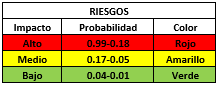
\includegraphics[scale=0.7]{32/img/tablaRiesgosInternos.png}
        \caption{Riesgos Internos}
        \label{fig:enter-label}
    \end{figure}
    %
    %
    \begin{figure}[H]
        \centering
        \includegraphics[scale=0.7]{32/img/tablaDescripciónDeRiesgos.png}
        \caption{Tabla Descripción de Riesgos}
        \label{fig:enter-label}
    \end{figure}
    
    %
    \subsubsection{Riesgos externas}
    
    Se les recuerda a los autores que los encabezados deben de estar conforme los solicita la guía del autor. De ahí se puede adaptar el trabajo para que sea más fácil de entender para el lector.
    Los encabezados organizan los temas sobre una base relacional y jerárquica. Por ejemplo, el título del documento es encabezado del texto principal porque todo el material posterior se relaciona y elabora sobre este tema. 
    
    \subsection{Determinación del tiempo estándar para que una persona competente realice el trabajo con marcha normal}
    %
    %
    Visualizar los siguientes diagramas
    %
    %
    \begin{figure}[H]
        \centering
        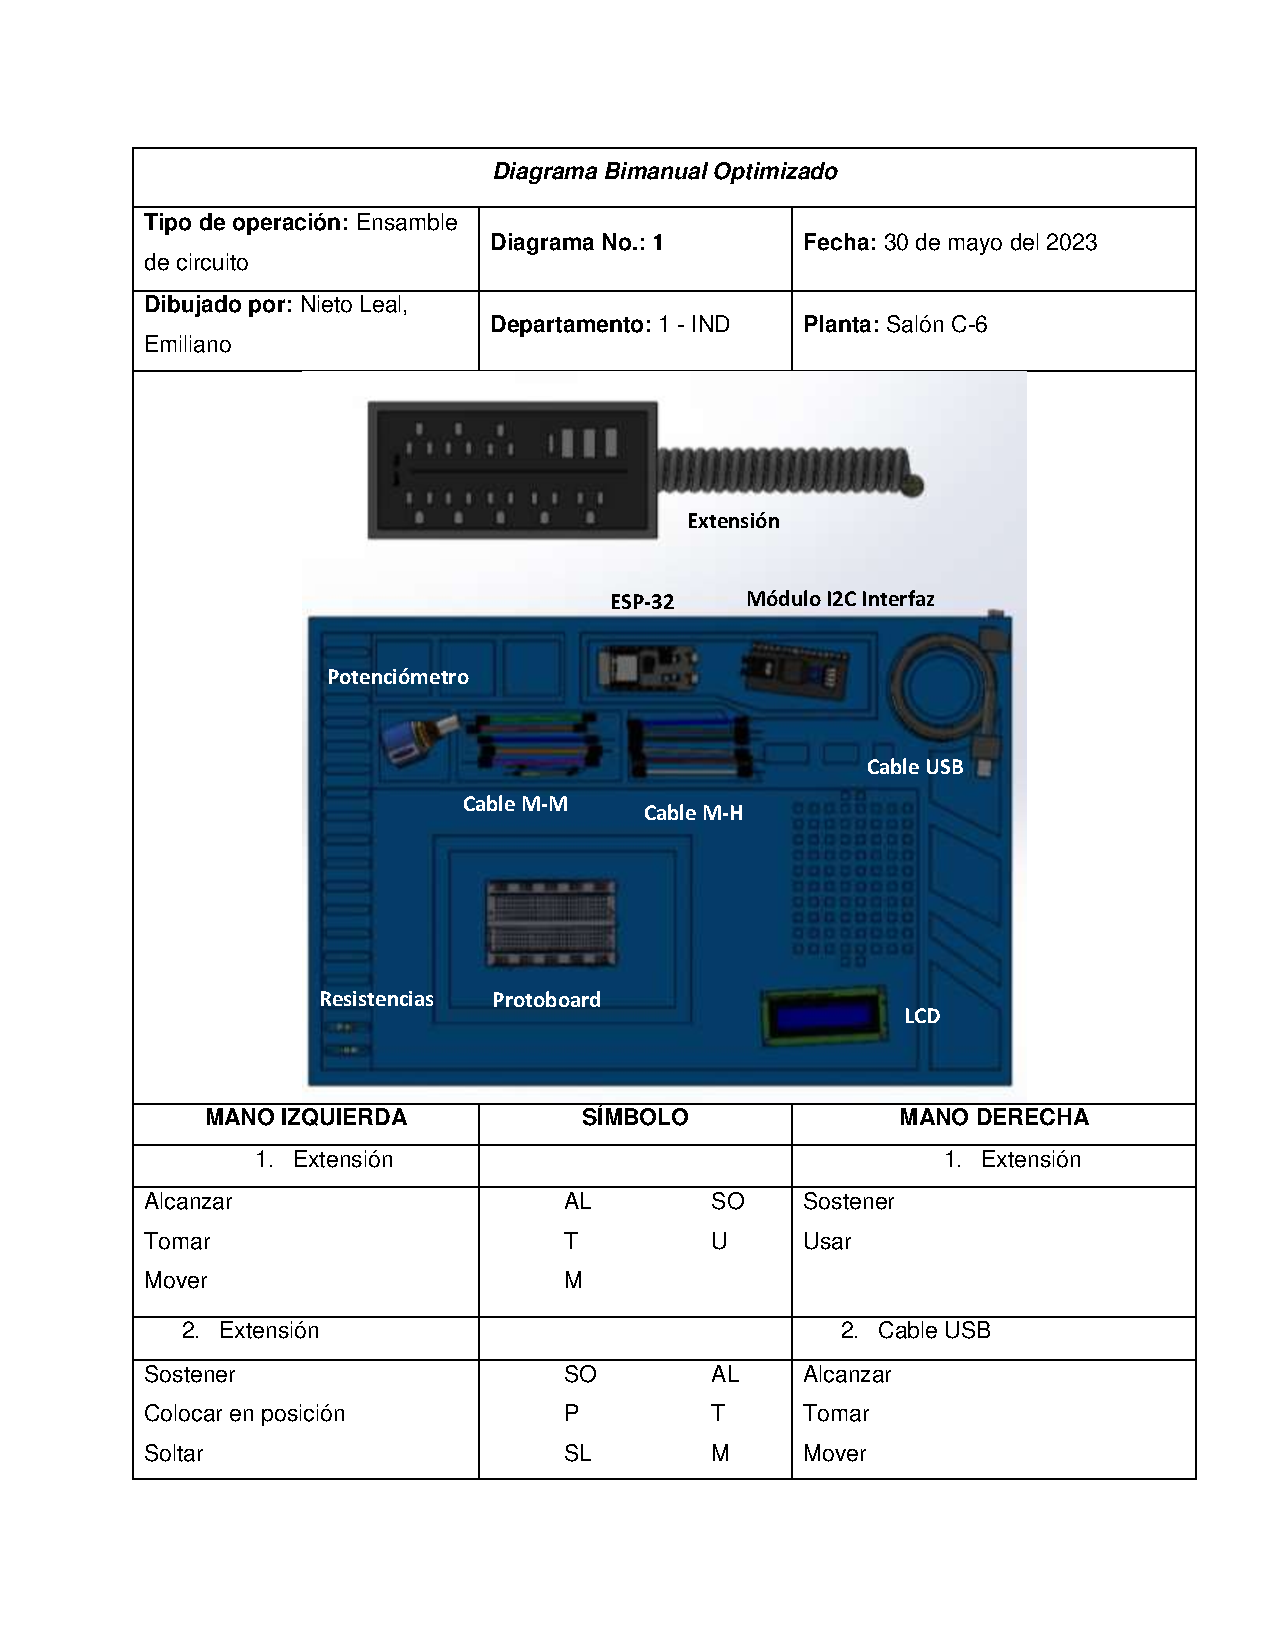
\includegraphics[scale=0.4]{32/img/diagramaBimanual.pdf}
        \caption{Diagrama Bimanual}
        \label{fig:enter-label}
    \end{figure}
    %
    %
    \begin{figure}[H]
        \centering
        \includegraphics[scale=0.4]{32/img/tablaAnálisisMTM.pdf}
        \caption{Análisi MTM}
        \label{fig:enter-label}
    \end{figure}
    %
    %
    \begin{figure}[H]
        \centering
        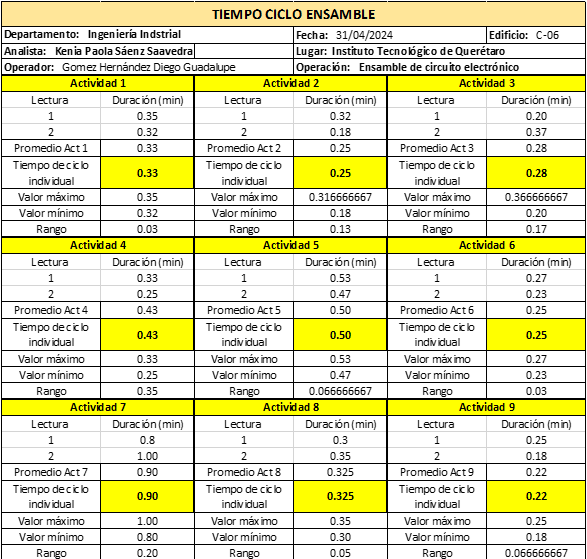
\includegraphics[scale=0.5]{32/img/tiempoCiclo1.png}
        \label{fig:enter-label}
        \centering
        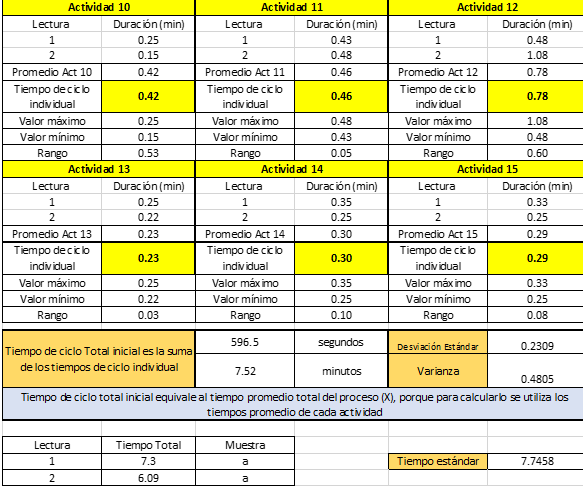
\includegraphics[scale=0.5]{32/img/tiempoCiclo2.png}
        \caption{Tabla Tiempo Ciclo}
    \end{figure}
    %
    %
    \begin{figure}[H]
        \centering
        \includegraphics[scale=0.5]{32/img/tiempoEstándar1.png}
        \label{fig:enter-label}
         \centering
        \includegraphics[scale=0.5]{32/img/tiempoestándar2.png}
         \centering
    \end{figure}
    %
    \begin{figure}[H]
        \includegraphics[scale=0.5]{32/img/tiempoEstándar3.png}
         \centering
        \includegraphics[scale=0.5]{32/img/tiempoEstándar4.png}
         \caption{Tabla Tiempo Estándar}
         \label{fig:enter-label}
    \end{figure}
    %
    %
    
    \section{Conclusiones}
    %
    %
    Al comienzo de este proyecto se estableció el objetivo de buscar la manera más económica de realizar el trabajo, esto desarrollado a través de un circuito electrónico realizando un estudio de tiempos y movimientos, apoyándonos de diferentes plataformas e integrando conocimientos adquiridos de otras materias durante los semestres cursados.
    Después de arduas semanas de trabajo no se pudo concluir totalmente este proyecto debido a algunas dificultades técnicas con algunos materiales, sin embargo si podemos llegar a la conclusión de que efectivamente se cumplió la Hipótesis; a través de un buen análisis de tiempos y movimientos, estudiando todos los factores que intervengan en un trabajo se puede obtener la manera más económica de realizar el trabajo, ya que con la eliminación de movimientos, la modificación de materiales, el uso de las 5´S y todas las metodologías que llevamos a la práctica, se reducen los tiempos y se aumenta la productividad  obteniendo como resultado la reducción de los costos.
    De igual manera podemos concluir que la mejor manera de determinar el tiempo estándar es a través de loa Sistemas de Tiempo Predeterminado, en este caso utilizamos el MTM (Medición de Tiempos Métodos) ayudándonos de un muestreo en conjunto con compañeros para poder normalizar la operación.
    Podemos decir sin duda, que la elaboración de este proyecto nos hace ampliar nuestra vista sobre cómo será nuestro desempeño en el campo laboral, el grado de dificultad que tenía este proyecto nos hizo retarnos tanto académicamente cómo personalmente, haciéndonos trabajando bajo presión durante los últimos días. A pesar de que no se concluyó totalmente, yo me quedo agradecida con la propuesta del profesor, pues aprendimos mucho en esta materia de Estudio del Trabajo II, sabiendo que podré aplicar estos nuevos conocimientos más adelante en otras materias y por supuesto en el campo laboral en un futuro.
    \section{Agradecimientos}
    
    Es importante darles su debido reconocimiento a los laboratorios, instituciones, organizaciones, entre otros que han sido participes para la culminación de este trabajo. También es importante mencionar, fondos, proyectos, becas, entre otros que se le han otorgado al o los autores para realizar el trabajo de investigación. Ejemplo: “Los autores agradecen al Concejo Nacional de Ciencia y Tecnología por los recursos otorgados…”
    
    
    

    % Ejemplo
    %  @Article{article,
    % 	author = "Author1 LastName1 and Author2 LastName2 and Author3 LastName3",
    % 	title = "Article Title",
    % 	volume = "30",
    % 	number = "30",
    % 	pages = "10127-10134",
    % 	year = "2013",
    % 	doi = "10.3389/fnins.2013.12345",
    % 	URL = "http://www.frontiersin.org/Journal/10.3389/fnins.2013.12345/abstract",
    % 	journal = "Frontiers in Neuroscience"
    % }
    
    % @book{book,
    %   author    = {Author Name}, 
    %   title     = {The title of the work},
    %   publisher = {The name of the publisher},
    %   address   = {The city},
    %   year      = 1993,
    % }
    
    % @incollection{chapter,
    %   author       = {Bauthor Surname}, 
    %   title        = {The title of the work},
    %   editor       = {Editor Name},
    %   booktitle    = {The title of the book},
    %   publisher    = {The name of the publisher},
    %   address      = {The city},
    %   year         = 2002,
    %   pages        = {201-213},
    % }
    
    % @InProceedings{conference,
    %   author = {Cauthor Name and Dauthor Surname and Fauthor LastName},
    %   title = {The title of the work},
    %   booktitle = {The title of the conference proceedings},
    %   year = 1996,
    %   publisher = {The name of the publisher},
    %   editor = {Editor Name1 and Editor Name2},
    %   pages = {41-50},
    % }
    
    % @book{cho,
    %   author       = {Gauthor Name1}, 
    %   title        = {The title of the work},
    %   publisher = {Country code and patent number},
    %   address      = {Patent Country},
    %   year = 2013
    % }
    
    % @book{patent,
    %   author    = {Hauthor Surname1}, 
    %   title     = {The title of the work},
    %   publisher = {Patent number},
    %   address   = {Patent country},
    %   year      = 2010,
    % }
    
    % % please use misc for datasets
    % @misc{dataset, 
    % 	author = "Author1 LastName1 and Author2 LastName2 and Author3 LastName3",
    % 	title = "Data Title",
    % 	year = "2011",
    % 	doi = "10.000/55555",
    % 	URL = "http://www.frontiersin.org/",
    % }
    
    \bibliographystyle{ieeetr}
    \bibliography{32/referencias}
    % 
    % 
    %%%%%%%%%%%%%%%%%%%%%%%%%%%%%%%%%%
    \appendix
    %%%%%%%%%%%%%%%%%%%%%%%%%%%%%%%%%%
    % 
    % 
    
    %%%%%%%%%%%%%%%%%%%%%%%%%%%%%%%%%%
    \appendix
    %%%%%%%%%%%%%%%%%%%%%%%%%%%%%%%%%%
    % 
    % 
    
    %%%%%%%%%%%%%%%%%%%%%%%%%%%%%%%%%%%%%%%%